\chapter{Reactive Behaviours}
\label{chap:reactive}

We are going to design a robot which could do multiple Braitenberg’s behaviours, which has four specific behaviour, they are love, aggression, fear and curious. 
Firstly, finding a good targeted object is very important. It needs to be easy to recognize while robot is swing on the floor. 
By several testing we have decided that a backpack is the best static targeted object to use in labs. Because it not only contains different unique features, but also the size of the object is suitable for camera to recognize. 
Before it starts doing behaviour, it needs to wonder around to find targeted objects. 
Once it has targeted objected in its bounding box, it starts the behaviour that we designate. 
For each unique behaviour, we need to consider circumstances for each one of them.

\section{Assumptions}

Several assumptions are made in our design of reactive behaviours.

\begin{enumerate}
    \item There is no obstacle between the object and the robot.
    \item There is only one object of interest in the environment.
\end{enumerate}


\section{System Design}

\subsection{Flow Chart}

The algorithm of reactive behaviour is shown in Figure \ref{fig:reactive}. After we initiate the robot, the robot will rotate itself to scan around the area until it finds the targeted object.  While RGBD camera successfully lock the object, it will put a blue bounding box at it, then it will further process the image that it has been read to make sure it is the real targeted object, at that time, bounding box will become red and it will process what behaviour task we have been given in our computer. 
After one behaviour has been finished, it will start the previous process again and wait for command.

\begin{figure}
\centering
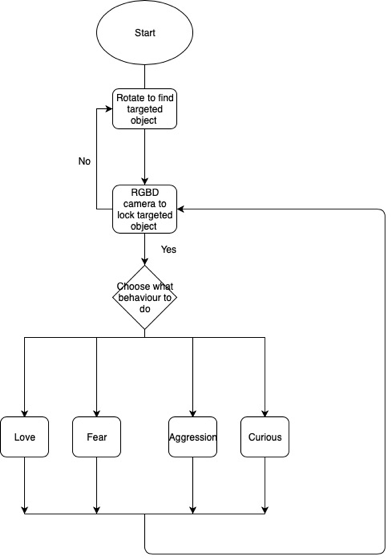
\includegraphics[width=0.5\textwidth]{reactive}
\caption{Flow Chart of the Mobile Robot with Reactive Behaviours.}
\label{fig:reactive}
\end{figure}

\subsection{Aggressive Behaviour}

Aggression means feelings of anger or antipathy resulting in hostile or violent behaviour; readiness to attack or confront in English, so we want robot to react some critical movements after it successfully located target. A significant accelerate of speed will be the key point of aggressive behaviour. It also should be stop from a safe distance to avoid collision. So, Depth sensor function in camera will be useful in this circumstance.

\begin{figure}
\centering
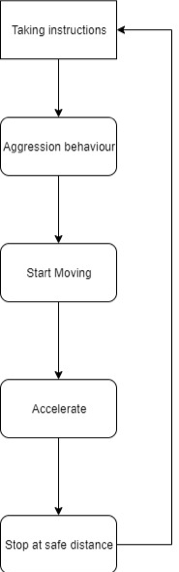
\includegraphics[width=0.3\textwidth]{aggressive}
\caption{Aggressive Behaviour.}
\label{fig:aggressive}
\end{figure}

Figure \ref{fig:aggressive} describes Aggressive Behaviour in details.
For Aggressive Behaviour, after robot taking instructions, it will initiate its motor to a stable speed, while depth camera has a reading that targeted object has beyond safe distance, it will centralise its direction towards object, then it will accelerate significantly towards targeted object. While depth camera has reading that it reached safe distance, the motor will stop to avoid collision to the target.

\subsection{Fear Behaviour}

In opposite to Aggression, fear behaviour should keep a distance from the target. So RGBD camera should be use as well. While robot has detected the targeted object, it firstly using depth camera to read distance between object and itself, then it will move backward in a significant speed. The speed should also decrease as the distance between targeted object increase.

\begin{figure}
\centering
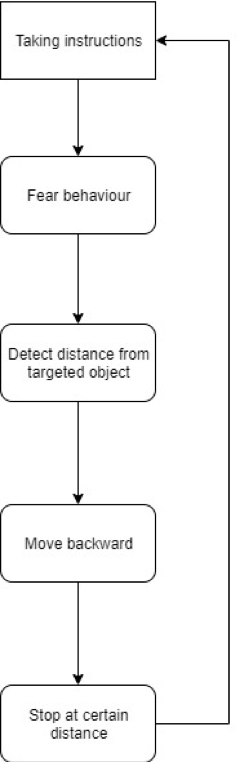
\includegraphics[width=0.3\textwidth]{fear}
\caption{Fear Behaviour.}
\label{fig:fear}
\end{figure}

Figure \ref{fig:fear} describes Fear Behaviour in details.
In contrast to Aggressive Behaviour, Fear is doing opposite movement, it also starts by wondering around. While targeted object has been detected and confirmed, it will quickly move backwards from the target. There is also a deceleration of speed that we have designed at this part, which means the farther away the robot is from the targeted object, the slower it moves.

\subsection{Curious Behaviour}

Curious means eager to know or learn something, as a robot with only movement physical function, we define curious as a movement that contains moving forward and moving backward constantly. While targeted object is detected in camera’s sight, it will seek if the target is at left side or right side, then it will move left forward or right forward correspondingly.

\begin{figure}
\centering
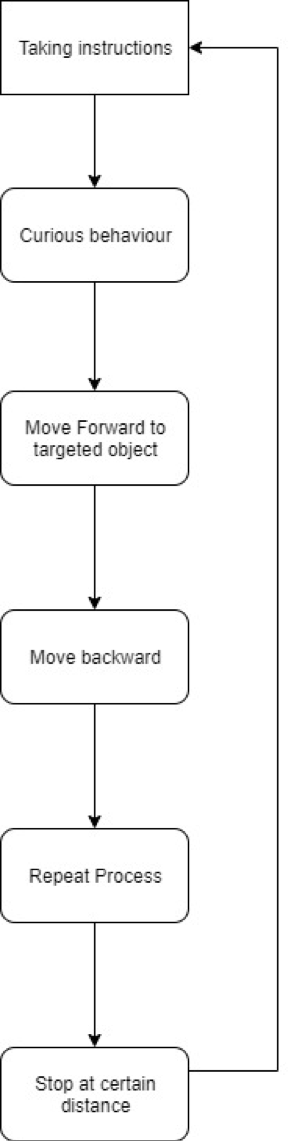
\includegraphics[width=0.3\textwidth]{curious}
\caption{Curious Behaviour.}
\label{fig:curious}
\end{figure}

Figure \ref{fig:curious} describes Curious Behaviour in details.
Curious Behaviour uses same direction recognition technique as ‘Love’ behaviour, by defining what location of targeted object that robot is facing; For example If targeted object is on left side of the robot, robot will move left forward towards the target, while it getting closer, it will moving backward, and moving towards the target again until it reaches the safe distance.

\subsection{Love Behaviour}

Love is hard to define for a simple physical movement robot since it’s an emotional vocabulary. We defined love as move slowly and shake its head while moving. When targeted object has been detected, it will turn left, then go forward a bit, then move right, forward a bit. It terminates the movement after reaching the safe distance from object.

\begin{figure}
\centering
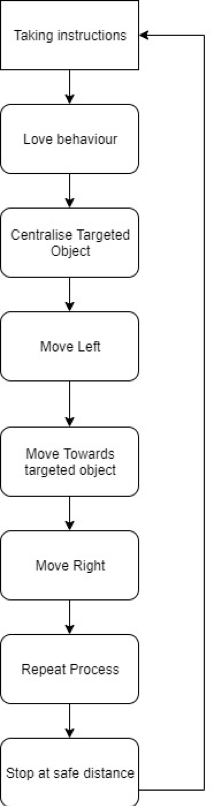
\includegraphics[width=0.3\textwidth]{love}
\caption{Love Behaviour.}
\label{fig:love}
\end{figure}

Figure \ref{fig:love} describes Love Behaviour in details.
When t robot is taking instructions of doing ‘Love’ behaviour, it will firstly find targeted object, after successfully put the bounding box on the targeted object, it will define whether object is on its left or on its right, then it will turn its direction to the opposite, then it will move forward a bit and turn its direction again, to do this movement is simply because wants robot to combine this series of movement, after-all the robot will shakes its head as he walks towards the target.

\section{Implementation}
Task 1 was to implement the Braitenberg behaviours which are love, fear, aggression and curiosity. 
Each of the behaviours the robot needs to first find the target we have specified. This is done within the process function which first calculates all the detected objects in the view of the camera. 

\begin{lstlisting}[language=Python]
detections = model(imgsized)
\end{lstlisting}

We then filter out the detections found to give us an array of only objects that we are interested in. 

\begin{lstlisting}[language=Python]
matching_detections = [d for d in detections[0] if d['label'] == int(label_widget.value)]
\end{lstlisting}

Finally, each detection has a confidence field which is used to show the confidence (0-1) that the object is the one we want. If the confidence is less than 0 (i.e. not our object) we draw a blue bounding box around it otherwise if the object is what we want, we draw a red bounding box around it. 

Additionally, we keep a count of the number of objects that the camera sees so we have a counter of all the objects on the left-hand side of the screen, centre of the screen and right-hand side of the screen. 

This is done with the following code:
\begin{lstlisting}[language=Python]
if (bbox[0]+bbox[2])/2 < 2/5.0:
                left_count = left_count + 1
            elif (bbox[0]+bbox[2])/2 > 3/5.0:
                right_count = right_count + 1
            else:
                center_count = center_count + 1
\end{lstlisting}

When the robot does not find the object we want, the robot does a 360 rotation (starting left or right depending on how many objects there are on that side, so if there are more objects on the right hand side, the robot will start turning  towards the right). Once the object has been detected, the emotion that has been selected will be executed.

A dropdown widget has been added to allow users to specify the behavior they want. By default this is set to love.

\subsection{Aggressive Behaviour}
The aggression behavior is implemented by first having the robot move towards the side of the screen that has the most objects. Once the target object has been located, the robot will move towards the object increasing its speed the closer it gets to the object. Once the robot has reached a distance of 1200 or less, the robot stops. The gradual speed up from slow to fast going to the object is how we have implemented aggression. 

The code for agression: 
   
\begin{lstlisting}[language=Python]
    if distance < 1200:
        robot.stop()
    elif left_count > right_count and left_count > center_count:
        robot.forward_left(max((5000-distance)/2500*2+0.3, 0.3))
    elif right_count > left_count and right_count > center_count:
        robot.forward_right(max((5000-distance)/2500*2+0.3, 0.3))
    else:
        robot.forward(max((2000-distance)/2000*2, 0.3))
\end{lstlisting}

The code shows how the robot stops if too close and how it moves left, right or center depending on what side of the screen the object is on. The speed is increased as the distance is shortened. 


\subsection{Fear Behaviour}
Fear is implemented by first havimg the robot robot move in the direction where there are the most objects (left, centre or right) then once it detects the target object and is less than 2500mm in distance, the robot goes backwards in reverse quckly. The robot can be observed to slow down the further away it is from the object. 

This is done with the following code:

\begin{lstlisting}[language=Python]
            if distance < 2500:
                robot.backward(max((3000-distance)/3000*2, 0.3))
\end{lstlisting}

We choose that 3000 is the max distance we can do this from and that the speed can range between 0-1. Thus this gives the affect of fear with the control of speed.


\subsection{Curious Behaviour}
For curiosity we have made the robot go towards the area that has the most amount of objects. This is because we believe that where there are more objects, the robot is more curious. The robot will stop if the distance between the object is less than 800mm otherwise it will either go left, right, or center depending on object count on that side. The code to see the behavior is in the curious function were a direction is specified and the movement happens accordingly. For the curious behavior we have made the robot go forward and backwards towards the target object once it has been located. 

\subsection{Love Behaviour}
The way love is implemented is once the robot has found the target object, the robot moves left, moves forward, moves right and then moves forward again. This results in the robot moving in a sort of short ziggzag fashion towards the object. This can be observed in the love function. Additionally, to keep the robot on track towards the object, in the process function we check if the distance is bigger than 100mm and depending on what side of the screen the most amount of objects are, we turn the robot towards that direction (i.e. if there are more objects on the left, we make the robot turn left). Once the robot reaches a safe distance of 900mm the robot stops. 

The love function:
\begin{lstlisting}[language=Python]
    def love():
        global love_flag
        if love_flag == 0:
            robot.left(0.5)
        elif love_flag == 1:
            robot.forward(0.3)
        elif love_flag == 2:
            robot.right(0.5)
        elif love_flag == 3:
            robot.forward(0.3);
        love_flag = (love_flag + 1) % 4
\end{lstlisting}

The love\_flag is used to keep track of the movement that had been performed. This is so that we can control the movement of the robot in stages.

\section{Test \& Analysis}

Our group test the task 1 in the computer master students Lab. In this Lab, we put the robots on the carpet. Because there are too many chairs and people. So, we decide to use the cup first. But is too small to recognize. Then we test the keyboard, but it still hard for robot’s camera to recognize. Finally, we decide to use the black bag as the object. Because it is big enough to be easy to recognize.


\subsection{Aggressive Behaviour}

When we test this function, after choosing the aggressive. The robot will approach target slowly. When it close to the object, the robot will accelerate significantly. In order not to damage the robot, we design to stop in front of the target. Instead of going randomly, we design the if the robot cannot find the object. The robot will rotate in place, until find the object.

\begin{figure}
\centering
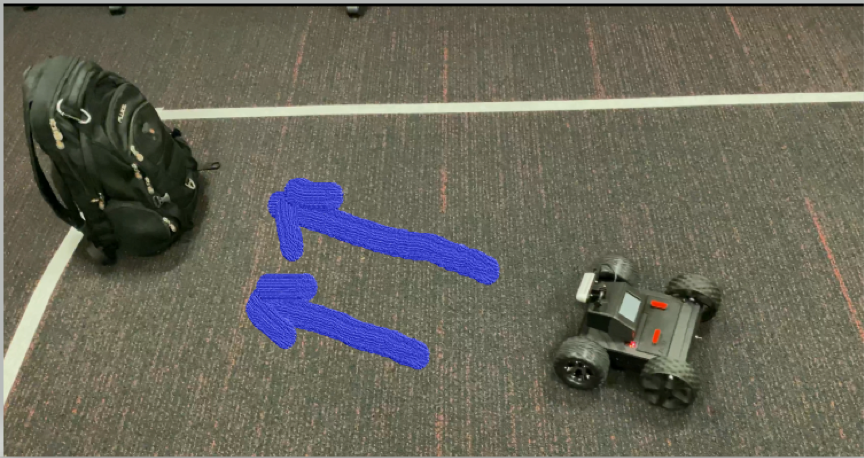
\includegraphics[width=0.8\textwidth]{aggressive-test}
\caption{Testing of Aggressive Behaviour.}
\label{fig:aggressive-test}
\end{figure}

From the capture in the video shown in Figure \ref{fig:aggressive-test}, we can find that the process of accelerate is very clearly. It can show this function is accomplished perfectly. During the test, we found that the need some distance to show this function obviously. 

\subsection{Fear Behaviour}

When we test this function, after choosing the fear. The robot will leave the object quickly. Just like the real fear. At first, we set the stop distance as 2500. During the test, the 2500 is too far away sometimes the camera will lose the object because the distance is too big, then the robot will rotate in place to find the object again. In order to this situation. We change the distance as 1800. 

\begin{figure}
\centering
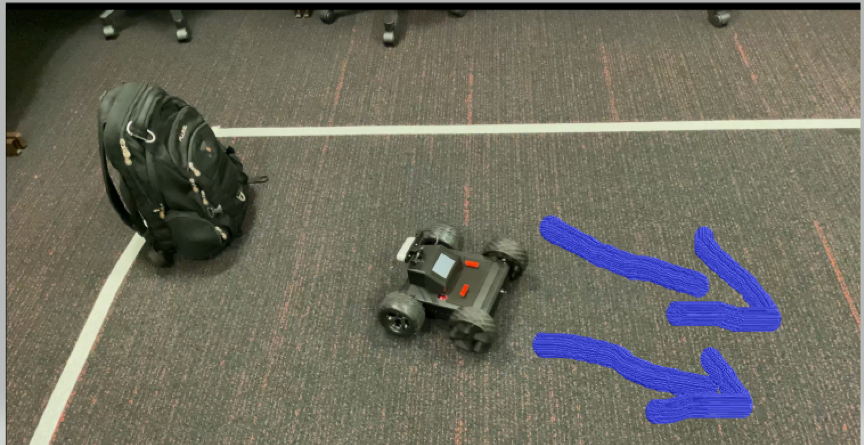
\includegraphics[width=0.8\textwidth]{fear-test}
\caption{Testing of Fear Behaviour.}
\label{fig:fear-test}
\end{figure}

From the capture in the video shown in Figure \ref{fig:fear-test}, we can find that the distance 1800 is pretty appropriate for the test. The leave process is obvious. The function is completely accomplished.

\subsection{Curious Behaviour}

When we test this function, after choosing the curious. The robot will find where is the object, then forward and backward during the forward process. There are some questions when we test this function. At first, we set the forward or backward speed to high. Then the camera also easy to lose the object. So, we turn down the speed. After that, the result is better than before.

\begin{figure}
\centering
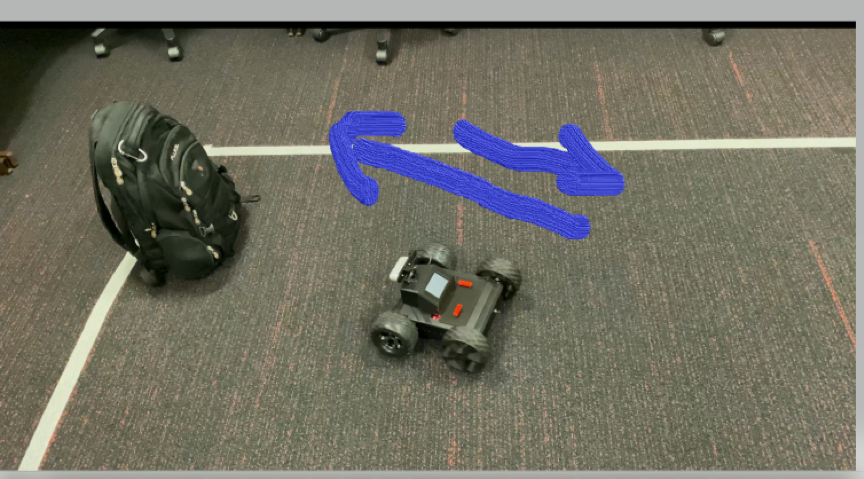
\includegraphics[width=0.8\textwidth]{curious-test}
\caption{Testing of Curious Behaviour.}
\label{fig:curious-test}
\end{figure}

From the capture in the video shown in Figure \ref{fig:curious-test}, the robot forward and backward and during this process, the camera still can get the object. So, this function is successful.


\subsection{Love Behaviour}


When we test this function, after choosing the love. The robot will find where is the object, then turn left and turn right, like shake the robot. During the test we find some question, the robot is hard to find the project during turn left and right. It is easy to lose the object when the process of making a turn. At first, we segment the frame to 3 part, left, right and center. Then we found it is easy to lose the object. So, we change the frame and segment it to 5 part. The left two parts as left. The middle part as the center. And the right two parts as the right. The robot turns left or turn right by in bounding box which part contain the most objects. After do this, the robot is better to find the object during the turning process.

\begin{figure}
\centering
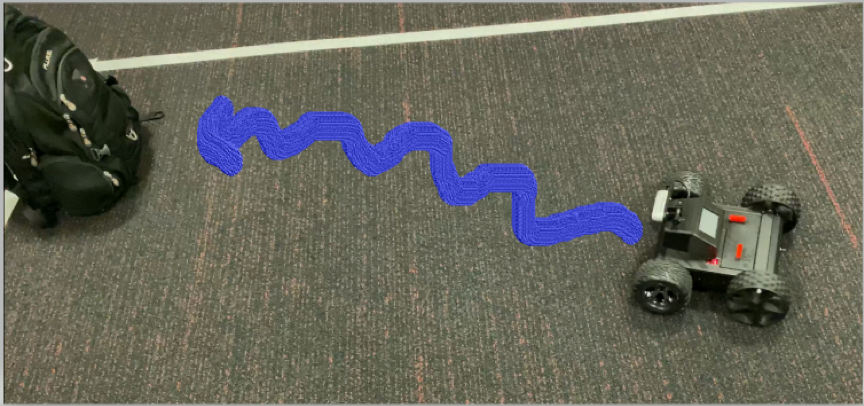
\includegraphics[width=0.8\textwidth]{love-test}
\caption{Testing of Love Behaviour.}
\label{fig:love-test}
\end{figure}

From the capture in the video shown in Figure \ref{fig:love-test}, we can find that the camera can recognize the object from beginning to the end. And perfectly complete the love function turn left and turn right during the forward process.

\subsection{Facing Backward to the Object}

In order to test the stability of the function. We also test some special situation not test before. For example, the robot is facing back to the object, side to the object and no object at all.

\begin{figure}
\centering
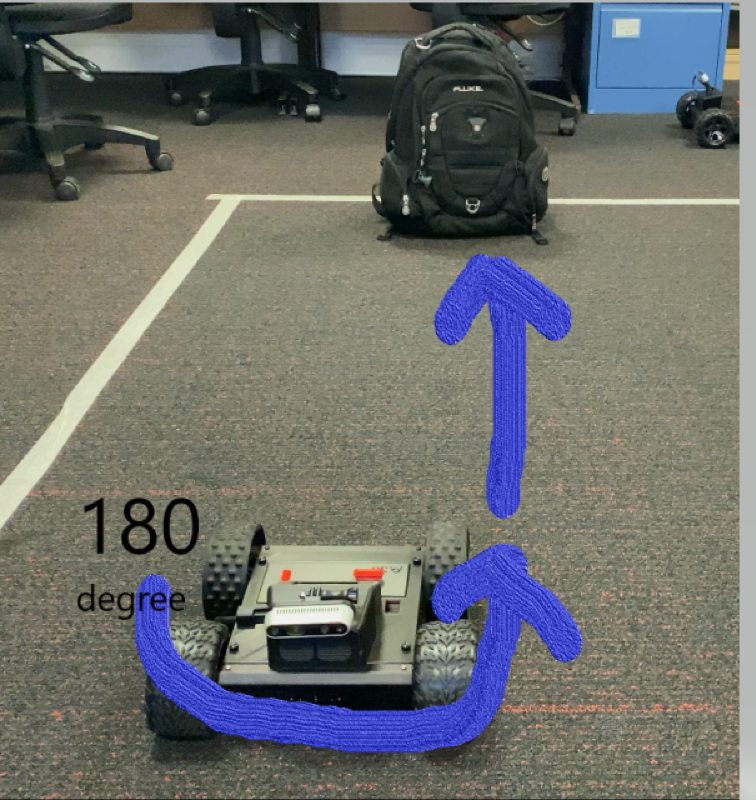
\includegraphics[width=0.8\textwidth]{back-test}
\caption{Testing of Facing Backward to the Object.}
\label{fig:back-test}
\end{figure}


In this situation, we put the black bag in the back of the robot, the robot will make a turn in place for about 180 degrees angle to find the object in the back of the robot. After find the object, the expected outcome is the same with the actual outcome. The robot can find the object quickly.

Just like the capture in the video shown in Figure \ref{fig:back-test}, we can find it can find the object in the back of the robot.

\subsection{Facing Sideways to the Object}

In this situation, we put the black bag in the side of the robot, the robot will make a turn in place for about 90degree angle to find the object in the side of the robot.

\begin{figure}
\centering
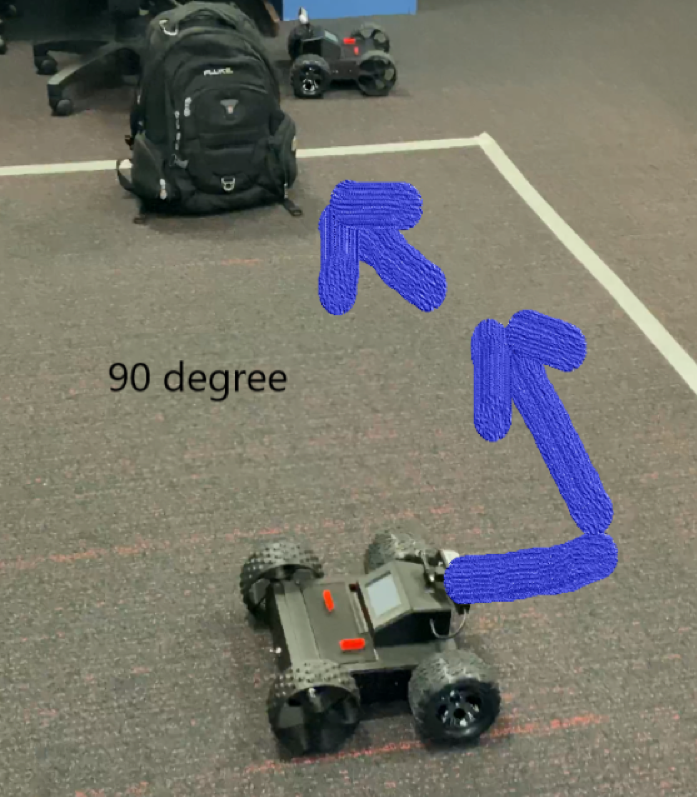
\includegraphics[width=0.8\textwidth]{side-test}
\caption{Testing of Facing Sideways to the Object.}
\label{fig:side-test}
\end{figure}

From this capture shown in Figure \ref{fig:side-test} we can find the robot can find the object in the side of the robot.

\subsection{No Object in the Environment}
In this situation, we do not put anything around the robot.

\begin{figure}
\centering
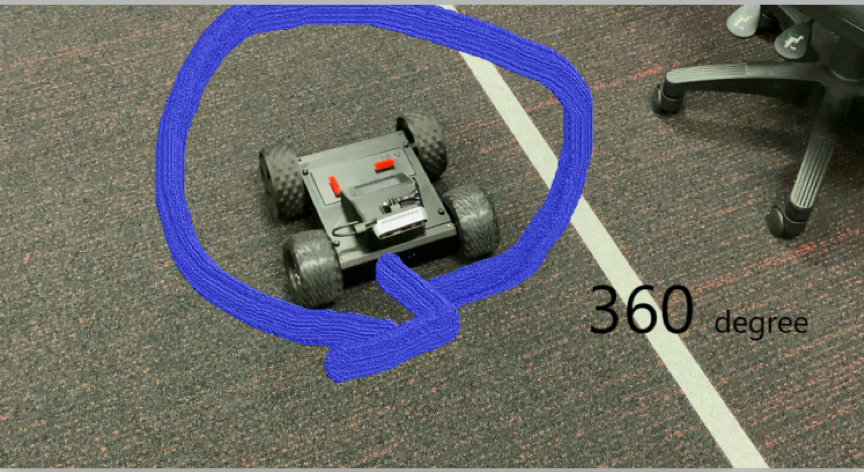
\includegraphics[width=0.8\textwidth]{no-test}
\caption{Testing of No Object in the Environment.}
\label{fig:no-test}
\end{figure}
 
From this capture shown in Figure \ref{fig:no-test}, we can find the outcome the robot is turning in place for 360 degrees again and again.
